% !TEX root =  main.tex
\section{Implementation}
\label{sec:implementation}

  %% TODO: Limites de l'approches
  % - ne traite pas les switch-case
  %    -> problème difficile (voir litt.)
  %    -> but ici : PoC ; pas indus.
  % - ne traite pas la récursivité
  %    -> relativement difficile (idem switch-case)
  %    -> pas possible (sans annotation) avec MC
  %    -> et pas MISRA
  % - pas intERprocédural
  %    -> quelles conséquences ? (sur approx. du slice)
  %    -> future work
  % - pas gestion de la mémoire
  %    -> quelles conséquences ?
  %    -> future work 

  %% Architecture:
  % - HARMLESS
  %    PowerPC Module (library and header files)
  %     modularity
  % - BEST (C++/LEMON)
  %    CFG reconstruction (from binary file)
  %    Program Slicing
  %      UPPAAL and Dot files

  \paragraph*{Architecture}{
    Our tool, \best\ for Binary Executable Slicing Tool, computes slices on
    binary executable files. 
    Its architecture is illustrated in Figure~\ref{fig:implem}.
    
  \begin{figure}[ht]
    \centering
    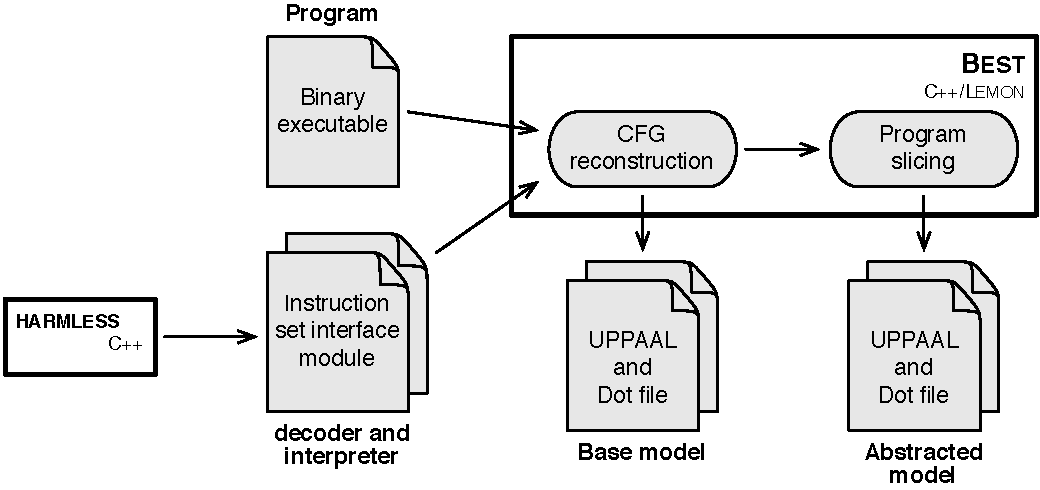
\includegraphics[scale=.5]{fig/workflow.pdf}
    \caption{Structure of the tool}
    \label{fig:implem}
  \end{figure}

    The decoding and interpretation of the binary files relies on a library
    generated by the \h\ toolchain~\cite{KBB12}. \h\ is an Hardware Architecture
    Description Language that is used to model a whole processor. In this study,
    we are only interested in the model of the instruction set. The \h\ compiler
    is primarily designed to generate either functional or cycle accurate
    simulators. We re-targeted it to extract static information of the
    instruction set. The library generated from \h\ can read a binary file
    (\texttt{.elf} format in our case) and give information about each
    instruction such as:
    \begin{itemize}
      \item the instruction mnemonic ;
      \item the memory locations that are read by the instruction ;
      \item the memory locations that are written by the instruction ;
      \item is the instruction a branch instruction? is it a conditional branch?
        what is its target (if it is statically defined)?
    \end{itemize}
    In this study we have used only the PowerPC instruction set, but
    \best\ is not architecture-dependent, thanks to this library.
    
    %% It handles binary executable files compiled for
    %% embedded targets based on PowerPC microprocessors. In order to do so
    %% properly it uses a library generated by \h~\cite{KBB12}, see
    %% figure~\ref{fig:implem}.\h\  is an architecture simulator
    %% generator based on a HDL. However, \best\ is a modular tool as we could use
    %% another library, as well generated by \h, to make our tool
    %% work with binary executable files compiled for another embedded target.
  
    Using this library, \best\ does a CFG reconstruction from a PowerPC binary
    executable file. Then it applies program slicing to compute the set of
    memory locations that should be in the model. The main output is an abstract
    model of the program that can be used to solve the WCET estimation problem
    with \textsc{Uppaal}. For validation and visualization purposes, the
    different models built along the computation can be exported as graphs or as
    timed automata in the \textsc{Uppaal} format~\cite{LPY97}.

  %% Implementation choices:
  % - Based on Kiss et al.
  % - C++
  % - LEMON

  \best\ is distributed in open-source\footnote{available at
    \url{https://github.com/TrampolineRTOS/BEST}}. To the best of our knowledge,
  there is no established program slicing tool for non-x86 binary code,
  especially in open-source. \best\ aims to fill this gap. It is implemented in
  C++. Apart from \h\, it relies on the graph manipulation library
  \textsc{Lemon}~\cite{DJK11}.
  
  %% Future work:
  % - Stack
  % - Interprocedurality

  \paragraph*{Limitations and Future work}

    The current version of \best\ has different limitations that we want to
    break in the near future. First, the computation of the abstraction is
    limited to the register file. The other levels of memory (stack words, all
    other parts of the volatile memory and non-volatile memory) are
    automatically excluded from the model. It will be straightforward to take
    into account the other levels by extending the technique used for the
    register file. The first step will be the analysis of the stack frame. Being
    able to track data dependencies between memory and registers through stack
    loads and stores will produce a more accurate model of the binary
    executable, and so more accurate WCET estimations.

    The second limitation is the limited support for programs with multiple
    procedures. The slice is currently computed on the PDG. It is not much of
    hard work to build the SDG and adapt the slicing algorithm because
    \best\ has been designed on structures and algorithms intended to produce
    inter-procedural slices. The main benefit of inter-procedural slicing
    resides on a more accurate slicing of procedure parameters i.e. even smaller
    slices.

    %% \best\ does not handle indirect branches. Indeed, statically resolve
    %% indirect branches is a hard and widely studied problem. Existing techniques
    %% only offers either under or over-approximations. Furthermore, the aim of our
    %% tool is to show that such an approach has a good potential in state-space
    %% reduction for model-checking based WCET computation and should be further
    %% studied. It is not intended to be complete and ready to be used
    %% industrially. Moreover, benchmark files we are using do not make use of such
    %% statements. One approach to statically tackle with indirect branches is
    %% based on constant propagation. Adding constant propagation to our tool could
    %% be a first step in resolving indirect branches and also a mean to reduce
    %% even more the set of memory locations that should be in the model.
